\documentclass[tikz]{standalone}
\usetikzlibrary{shapes.geometric,calc}

\begin{document}
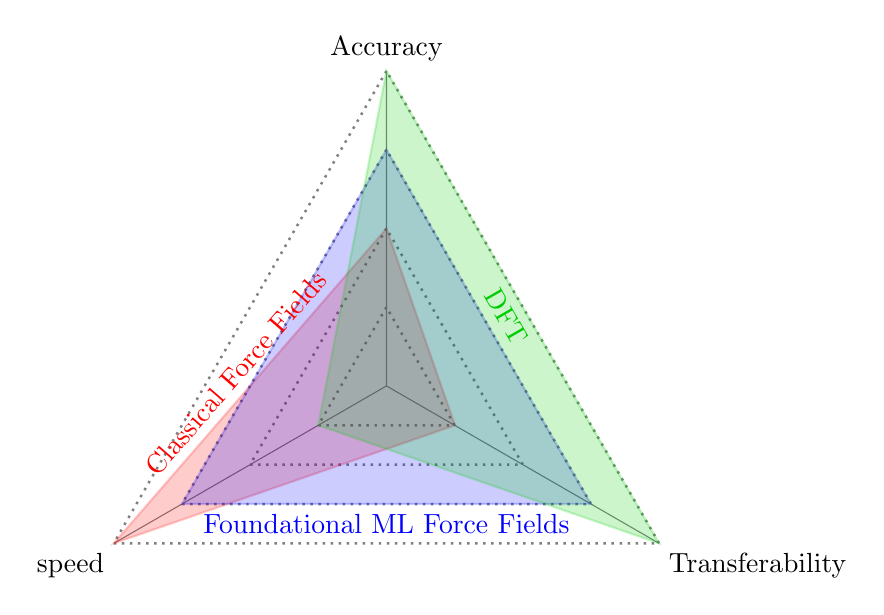
\begin{tikzpicture}
  % Define named coordinates
  \coordinate (origin) at (0,0);
  \coordinate (acc) at (0,4);
  \coordinate (speed) at (-3.464,-2);
  \coordinate (transfer) at (3.464,-2);
  % Define the axes
  \draw[gray] (origin) -- (acc) (origin) -- (speed) (origin) -- (transfer);
  % Draw the triangles
  \foreach \r in {1,2,3,4}
  {
    \draw[dotted,gray,line width=0.9pt] (0,\r) -- (-0.866*\r,-0.5*\r) -- (0.866*\r,-0.5*\r) -- cycle;
  }
  % Label the axes
  \node[anchor=south] at (acc) {Accuracy};
  \node[anchor=north east] at (speed) {speed};
  \node[anchor=north west] at (transfer) {Transferability};
  % Plot the shapes
  \draw[red, thick, fill=red, opacity=0.2] (0,2) coordinate (CFFACC) -- (speed) -- (.87,-.5) -- cycle;
  \draw[blue, thick, fill=blue, opacity=0.2] (0,3) -- (-2.598,-1.5) -- (2.598,-1.5) -- cycle;
  \draw[green!80!black, thick, fill=green!80!black, opacity=0.2] (acc) -- (-0.866,-0.5) -- (transfer) -- cycle;
  % Add rotated legend labels inside the shapes
  \node[red, anchor=south, rotate=49] at ($(speed)!0.5!(CFFACC)$) {Classical Force Fields};
  \node[blue, anchor=south] at ($(speed)!0.5!(transfer)$) {Foundational ML Force Fields};
  \node[green!80!black, anchor=center] at ($(acc)!0.5!(transfer)$) [anchor=north, rotate=-60] {DFT};
\end{tikzpicture}
\end{document}
